 \documentclass[12pt]{beamer}
%\documentclass{beamer}
%\usepackage[pdftex]{graphicx}

% \usepackage{subfigure}
% \usepackage{caption}
% \usepackage{epstopdf}
\usepackage{tikz}
\usepackage[utf8x]{inputenc}
\usepackage{default}
%\usepackage{enumitem}
\usepackage{subcaption}
\usetheme{default}
\usecolortheme{lily}
%\usecolortheme{beaver}
\useinnertheme{rectangles}
\useoutertheme{default}
\usepackage{mathrsfs}
\usepackage{mathtools}
\usepackage{color}
\setbeamerfont{frametitle}{size=\Large,series=\bfseries}

\usepackage{hyperref}
\hypersetup{
    colorlinks=true,
    linkcolor=blue,
    filecolor=magenta,      
    urlcolor=cyan,
}

\usepackage{graphicx}
% \setbeamertemplate{footline}%{infolines theme}
% {
% \leavevmode%
% \hbox{%
% \begin{beamercolorbox}[wd=.333333\paperwidth,ht=2.25ex,dp=1ex,center]{author in head/foot}%
% \usebeamerfont{author in head/foot}\insertshortauthor%~~(\insertshortinstitute)
% \end{beamercolorbox}%
% \begin{beamercolorbox}[wd=.333333\paperwidth,ht=2.25ex,dp=1ex,center]{title in head/foot}%
% \usebeamerfont{title in head/foot}\insertshorttitle
% \end{beamercolorbox}%
% \begin{beamercolorbox}[wd=.333333\paperwidth,ht=2.25ex,dp=1ex,right]{date in head/foot}%
% \usebeamerfont{date in head/foot}\insertshortdate{}\hspace*{2em}
% \insertframenumber{} / \inserttotalframenumber\hspace*{2ex}
% \end{beamercolorbox}}%
% \vskip0pt%
% }

%%%%%%%%%
\definecolor{tublu}{RGB}{87, 6, 140}
\definecolor{tublucomp}{RGB}{226, 225, 221}

%\setlist[description]{font=\normalfont\textcolor{tublu}}

\setbeamertemplate{blocks}[default]%[shadow=false]
\setbeamercolor{block body}{bg=tublucomp}%{bg=normal text.bg!92!black}
\setbeamercolor{alerted text}{fg=tublu} 
\setbeamercolor{itemize item}{fg=tublu}
\setbeamercolor{title}{fg=tublu}
\setbeamercolor{frametitle}{fg=tublu}
\setbeamercolor{structure}{fg=tublu}

%\usefonttheme{serif}
\setlength{\parindent}{0pt} 


\newtheorem{trm}{Theorem}[section]
\newtheorem{lem}[trm]{Lemma}
\newtheorem{prop}[trm]{Proposition}
\newtheorem{cor}[trm]{Corollary}
\newtheorem{con}[trm]{Conjecture}
\newtheorem*{cons}{Consequence}
\theoremstyle{definition}
\newtheorem{de}[trm]{Definition}
\newtheorem{rem}{Remark}
\newtheorem*{exa}{Example}

\renewcommand{\d}{\,\mathrm{d}}
\newcommand{\e}{\mathrm{e}}
\renewcommand{\Re}{\operatorname{Re}}
\renewcommand{\Im}{\operatorname{Im}}
\newcommand{\spn}{\operatorname{span}}
\newcommand{\ii}{\mathrm{i}}
\newcommand{\R}{\mathbb{R}}
%\setbeamertemplate{footline}[page number]


\numberwithin{equation}{section}
\setcounter{section}{21}


%%%%%%%%%%%%%%%%%%
%\titlegraphic{\includegraphics[height=8mm]{nyu_short_color.png}}
\title{{\bf The Maths behind Bitcoin }}
\date{April 14, 2018}
\author{Georg Stadler, Dominik Stuerzer \\ Courant Institute, NYU}

\begin{document}


\begin{frame}
\maketitle
\end{frame}


\begin{frame}{Overview}
  \begin{itemize}
  \item What are cryptocurrencies? What is bitcoin?\\[3ex]
    \pause
  \item How is it different from other currencies, e.g., \$ or EUR? \\[1ex]
    \pause
    \begin{itemize}
      \item It's decentralized, distributed and anonymous.\\[1ex]
    \end{itemize}
    \pause
  \item Does it have real value?
    \href{https://www.coindesk.com/price/}{Let's take a look\ldots}\\[3ex]
    \pause
  \item Where does it come from?\\[3ex]
    \pause
  \item How do payments work?
  \end{itemize}
\end{frame}

\begin{frame}
\frametitle{Virtual currencies}
Alice, Bob and Charlie hang out and exchange money frequently (e.g.~pay for dinner, go to the movies, \ldots):
\begin{itemize}
\item Alice pays Bob 20\$
\item Bob pays Charlie 30\$
\item Alice pays Charlie 5\$
\item Charlie pays Bob 15\$
\item \ldots
\end{itemize}
Inconvenient to exchange cash all the time!

\medskip

\textbf{Solution:} Keep a communal ledger!
\end{frame}

\begin{frame}
\frametitle{The Blockchain}
\textbf{Blockchain:} History of all transactions. This is the \underline{Ledger}!\\
\textbf{Blocks:} The building blocks of the Blockchain.


%\begin{tikzpicture}
%   \draw (0,0)  rectangle (2.5,1.5);
%   \draw (0,1) node[right] {A$\to$B: 5\$};
%   \draw (0,0.5) node[right] {A$\to$C: 10\$};
%   \draw (3,0)  rectangle (5.5,1.5);
%   \draw (3,1) node[right] {B$\to$A: 2\$};
%   \draw (3,0.5) node[right] {C$\to$B: 5\$};
%   \draw (6,0)  rectangle (8.5,1.5);
%   \draw (6,1) node[right] {B$\to$C: 4\$};
%   \draw (6,0.5) node[right] {A$\to$C: 3\$};
%   \draw[->] (2.55, 0.75) -- (2.95,0.75);
%   \draw[->] (5.55, 0.75) -- (5.95,0.75);
%   
%\end{tikzpicture}
\begin{figure}
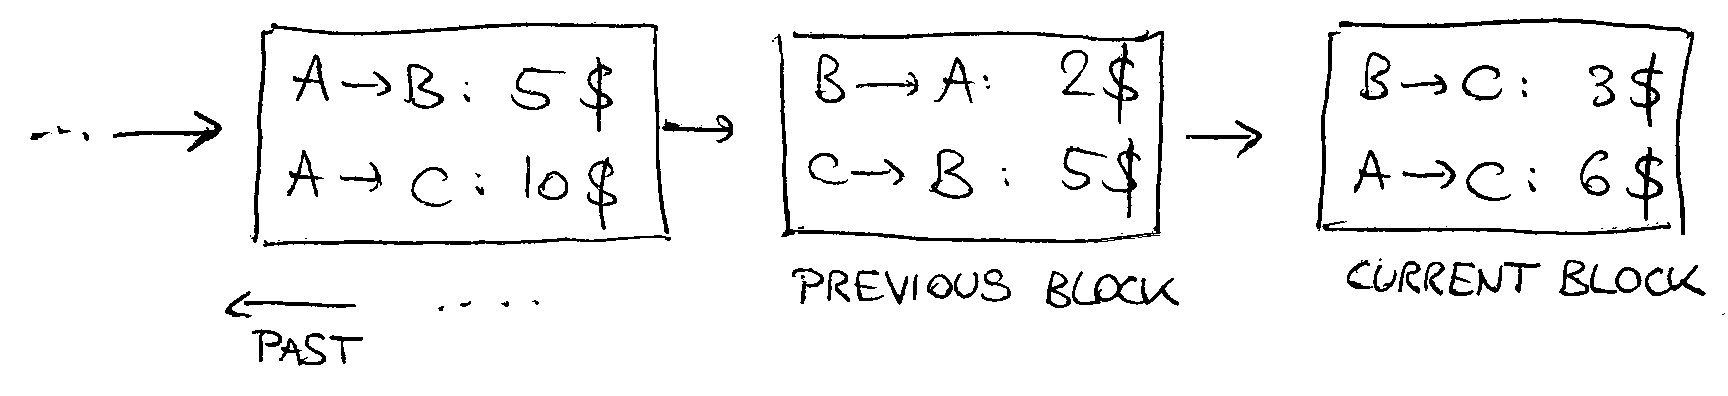
\includegraphics[scale=0.2, trim = {45mm 0mm 0mm 0mm}]{fig1}
\end{figure}
\end{frame}

\begin{frame}
\frametitle{Linking the blocks together}
Every block contains the \emph{hash} (\#) of the previous block:

\begin{figure}
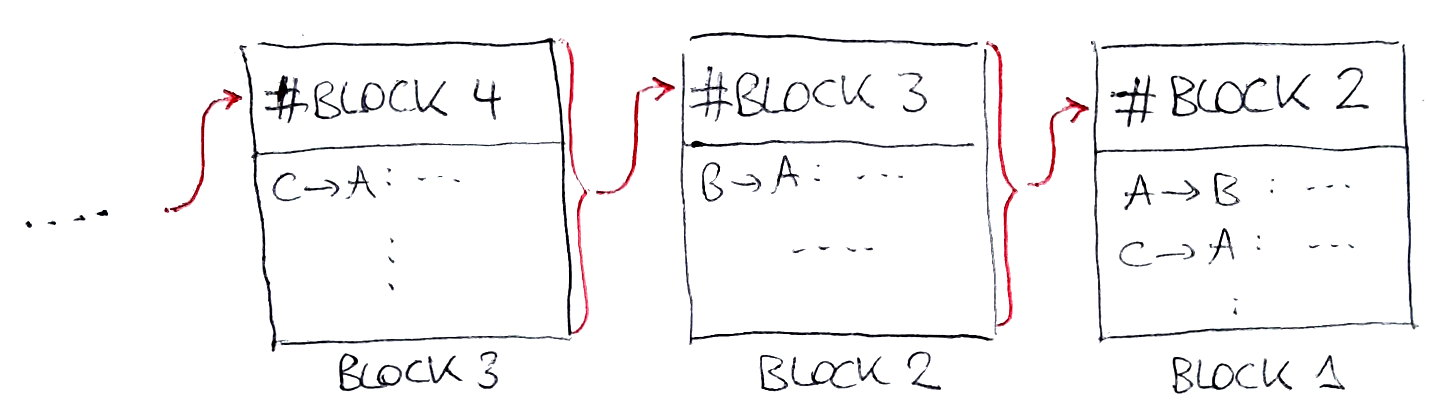
\includegraphics[scale=0.28, trim = {100mm 0mm 0mm 0mm}]{fig2.jpg}
\end{figure}
\pause
Change a previous block $\Rightarrow$ Re-compute all later hashes!

\end{frame}

\begin{frame}
\frametitle{Susceptibility to Fraud}
\underline{How to `steal' 100~BTC?}\\ \pause $\to$ fake the entire history of the 100~BTC! \\$\to$ recalculate all hashes in the Blockchain.
\begin{figure}
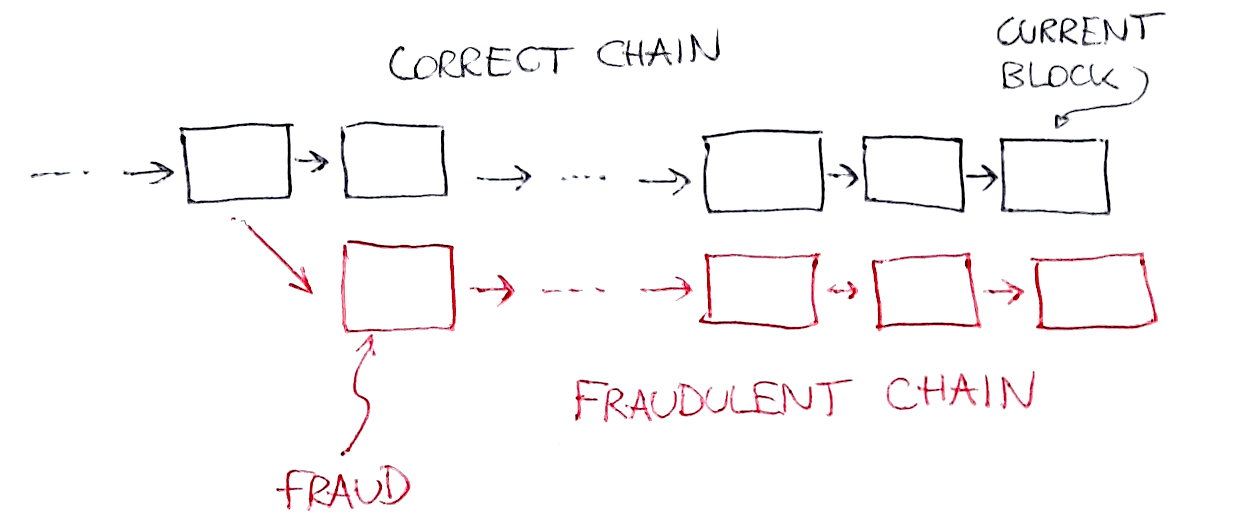
\includegraphics[scale=0.28, trim = {30mm 0mm 0mm 20mm}]{fig3}
\end{figure}
\pause
Which is the correct chain?
\end{frame}

\begin{frame}
\frametitle{Proof of Work}
\only<1>{\textbf{Answer:} Make hash computations hard!\\$\to$ recalculation of all hashes infeasible.}
\only<2->{
\textbf{Nounce:} Extra bits appended to each block.
\begin{figure}
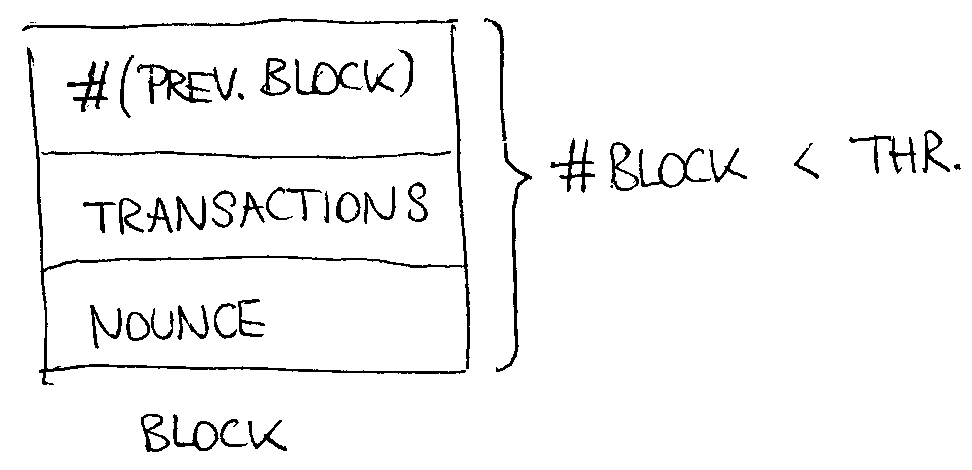
\includegraphics[scale=0.25]{fig4}
\end{figure}
\textbf{Mining:} \underline{Guess} nounces until \#(block) $<$ threshold.
}
\end{frame}


\begin{frame}
\frametitle{Mining}
\textbf{Mining:} \underline{Guess} nounces until \#(block) $<$ threshold.

\begin{figure}
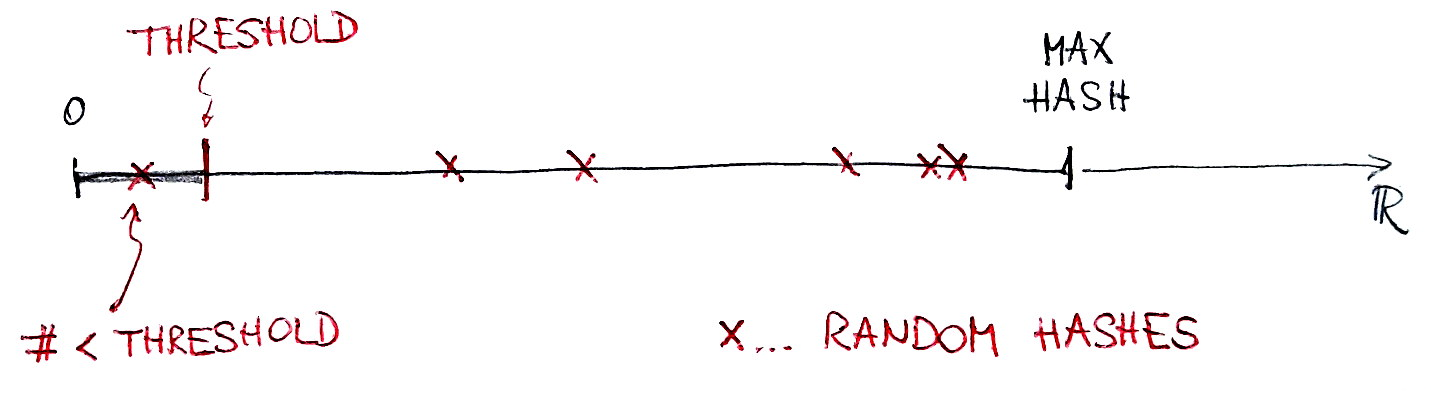
\includegraphics[scale=0.28, trim = {30mm 0mm 0mm 0mm}]{fig5}
\end{figure}
Millions of computers compete to complete the next block.\\
\underline{Threshold is small:} It takes all computers $\sim$10 minutes to find correct nounce.
\end{frame}

\begin{frame}
\frametitle{The Mining Game}
\textbf{Can you guess the nounce before others do?}
\end{frame}

\begin{frame}
\frametitle{Why is this safe?}
A \underline{valid} block in the blockchain:
\begin{itemize}
\item Contains \#(previous block).
\item \#(block) $<$ threshold.
\end{itemize}
\bigskip

\textbf{A fraudster against the world}
\begin{itemize}
\item A fraudster needs to \underline{re-calculate all nounces} \& hashes.
\item It took millions of computers \emph{10 minutes per block} to find a valid nounce.
\item $\Rightarrow$ fraudster can never catch up!
\end{itemize}
\end{frame}

\end{document}
